
\documentclass[ucs]{beamer}

\usetheme{GSyC}
%\usebackgroundtemplate{\includegraphics[width=\paperwidth]{gsyc-bg.png}}


\usepackage[spanish]{babel}
\usepackage[utf8x]{inputenc}
\usepackage{graphicx}
\usepackage{amssymb} % Simbolos matematicos
\usepackage{enumerate}


% Metadatos del PDF, por defecto en blanco, pdftitle no parece funcionar
   \hypersetup{%
     pdftitle={DevOps},%
     %pdfsubject={Diseño y Administración de Sistemas y Redes},%
     pdfauthor={GSyC},%
     pdfkeywords={},%
   }
%


% Para colocar un logo en la esquina inferior de todas las transpas
%   \pgfdeclareimage[height=0.5cm]{gsyc-logo}{gsyc}
%   \logo{\pgfuseimage{gsyc-logo}}


% Para colocar antes de cada sección una página de recuerdo de índice
%\AtBeginSection[]{
%  \begin{frame}<beamer>{Contenidos}
%    \tableofcontents[currentframetitle]
%  \end{frame}
%}


%\newboolean{detallado}
%\setboolean{detallado}{false}
%\newcommand{\opcional}[1]{\ifthenelse{\boolean{detallado}}{#1}{}}


\definecolor{darkred}{rgb}  {1.0, 0.0, 0.0}
\definecolor{darkgreen}{rgb}{0.0, 0.4, 0.0}
\definecolor{darkblue}{rgb} {0.0, 0.0, 0.8}

% for resalted text
\newcommand{\res}[1]{\textcolor{darkred}{#1}}
% for different text
\newcommand{\dif}{\textsl}
% for reserved words
\newcommand{\rw}[1]{\textrm{\textbf{#1}}}
% for commands
\newcommand{\com}[1]{\textrm{\textbf{#1}}}






\begin{document}

% Entre corchetes como argumento opcional un título o autor abreviado
% para los pies de transpa
\title[DevOps]{DevOps}

%\subtitle{Diseño y Administración de Sistemas y Redes}
\author[GSyC]{Escuela Técnica Superior de Ingeniería de Telecomunicación\\
Universidad Rey Juan Carlos}
\institute{gsyc-profes (arroba) gsyc.urjc.es}
\date[2017]{Noviembre de 2017}



%% TÍTULO
\begin{frame}
  \titlepage
  % Oportunidad para poner otro logo si se usó la opción nologo
  % \includegraphics[width=2cm]{logoesp}  
\end{frame}



%% LICENCIA DE REDISTRIBUCIÓN DE LAS TRANSPAS
%% Nota: la opción b al frame le dice que justifique el texto
%% abajo (por defecto c: centrado)
\begin{frame}[b]
\begin{flushright}
{\tiny
\copyright \insertshortdate~\insertshortauthor \\
  Algunos derechos reservados. \\
  Este trabajo se distribuye bajo la licencia \\
  Creative Commons Attribution Share-Alike 4.0\\
}
\end{flushright}  
\end{frame}



%% ÍNDICE
\begin{frame}
  \frametitle{Contenidos}

%\begin{tiny}
  \tableofcontents
%\end{tiny}

\end{frame}


\section{Definición}
%%---------------------------------------------------------------
\begin{frame}[fragile]
%\subsection{¿Qué es DevOps?}
\frametitle{Definición de DevOps}
\emph{DevOps} 
es un término acuñado por Andrew Shafer y Patrick Debois
en la conferencia de desarrollo \emph{Agile} del año 2008

Se origina con
la composición de dos palabras:

\begin{itemize}
\item
\emph{Development} 

Desarrollo, programación de software en sentido amplio, esto es, análisis, diseño, codificación y prueba

\item
\emph{Operations} 

Operaciones, explotación del software, puesta en producción, uso real
\end{itemize}


Definición de
Bass, Weber y Zhu \verb|[4]|:

\emph{DevOps is a set of practices intended to reduce the time between committing a change to a system and the change being placed into normal production, while ensuring high quality}

\end{frame}




%%---------------------------------------------------------------
\begin{frame}[fragile]
\frametitle{}
Definición de Davis y Daniels \verb|[2]|:

\emph{Devops is a cultural movement that changes how individuals think about their work,
values the diversity of work done, supports intentional processes that accelerate the
rate by which businesses realize value, and measures the effect of social and technical
change. It is a way of thinking and a way of working that enables individuals and
organizations to develop and maintain sustainable work practices. It is a cultural
framework for sharing stories and developing empathy, enabling people and teams to
practice their crafts in effective and lasting ways} 


\end{frame}
%%----------------------------------------------
\begin{frame}[fragile]

Definición de Huttermann \verb|[1]|:


\emph{DevOps is a mix of patterns intended to improve collaboration between development and
operations. DevOps addresses shared goals and incentives as well as shared processes
and tools. Because of the natural conflicts among different groups, shared goals and
incentives may not always be achievable. However, they should at least be aligned with
one another}

\end{frame}


%%---------------------------------------------------------------
\begin{frame}[fragile]
\frametitle{}
Aquí lo definiremos como

  \begin{verbatim}
Grupo de técnicas que buscan optimizar el trabajo 
conjunto de desarrolladores de software y administradores 
de sistemas
  \end{verbatim}


\begin{itemize}
\item
Optimizar: que sea rápido, sencillo, barato, de calidad y sin conflictos
\end{itemize}


Estas \emph{técnicas} se agrupan en dos grandes categorías

\begin{itemize}
\item
Culturales, políticas, organizativas. Referidas a la interacción entre personas

\item
Herramientas software
\end{itemize}

Las segundas son importantes, pero las primeras, más

\end{frame}



%%---------------------------------------------------------------
\begin{frame}[fragile]
\frametitle{}


Hay algunas cosas relativamente claras:
\begin{itemize}
\item
Qué es 
\emph{DevOps} 

\item
Qué no es 
\emph{DevOps} 

\item
Qué problemas se quieren solucionar

\item
Qué objetivos se buscan

\item
Lo relativa a herramientas 
software

\end{itemize}


Lo que no está tan claro es \emph{cómo}.
\emph{DevOps} es una disciplina compleja
\begin{itemize}
\item
Organizar el trabajo de personas es difícil. No se aprende en un libro. Lo que
puede valer en un entorno, puede ser inaplicable en otro
\end{itemize}

\end{frame}



%%---------------------------------------------------------------
\begin{frame}[fragile]
%\subsection{¿Qué NO es DevOps?}
\frametitle{¿Qué NO es DevOps? (1)}

\begin{itemize}
\item
%hutterman pg 6
\emph{DevOps}
no significa que desaparezca la frontera
entre desarrollo y producción

\item
No significa que los desarrolladores controlen el software en producción

\item
No significa que los administradores editen el código fuente

\item
\emph{DevOps}
nunca debería ser un departamento en una empresa, ni un cargo.
No tiene sentido hablar de \emph{Ingeniero DevOps}

\item
No significa que una sola persona desarrolle y opere

\begin{itemize}
\item
Excepto tal vez en empresas muy pequeñas
\end{itemize}

\item
No significa que una persona trabaje por dos (y cobre por una)
\end{itemize}
\end{frame}

%%---------------------------------------------------------------
\begin{frame}[fragile]
\frametitle{¿Qué NO es DevOps? (2)}
\begin{itemize}
\item
\emph{DevOps}
no es una herramienta software.
Tienen su utilidad, pero ni son suficientes ni son imprescindibles

\item
\emph{DevOps}
no es una certificación. No es una metodología concreta y única que
se pueda enseñar, que se pueda seguir y de la que uno se pueda examinar

\end{itemize}
\end{frame}

\section{Desarrollo Ágil}
%%---------------------------------------------------------------
\begin{frame}[fragile]
\frametitle{Desarrollo Ágil}
\emph{DevOps}
está muy ligado con el desarrollo de software
\emph{agile}
(\emph{ágil}), proviene de la misma comunidad,
tiene objetivos muy similares

\begin{itemize}
\item
Podemos considerar
\emph{DevOps}
una extensión del moviento \emph{agil} a la explotación
del software, no solo a su desarrollo
\end{itemize}
\end{frame}



%%---------------------------------------------------------------
\begin{frame}[fragile]
\frametitle{Modelo de desarrollo de softare en cascada}

El desarrollo en cascada
cascada (\emph{waterfall}) es el tradicional, generalmente aceptado y prácticamente único hasta los
años 1990

Formado por pasos que se siguen secuencialmente, de forma rígida, uno tras otro, sin vuelta atrás.

    \begin{enumerate}
    \item
Análisis de requerimientos
    \item
Diseño
    \item
Desarrollo (programación)
    \item
Prueba
    \item
Despliegue
    \item
Mantenimiento
    \end{enumerate}
\end{frame}


%%---------------------------------------------------------------
\begin{frame}[fragile]
\frametitle{Desarrollo Ágil}

En los años 1990 empiezan a aparecer diversas metodologías de
desarrollo de software que cuestionan el modelo en cascada


\begin{itemize}
\item
\emph{rapid application development,
the unified process,
dynamic systems development method (DSDM),
scrum,
extreme programming (XP),
feature-driven development}
\end{itemize}


En 2001 se publica el
\emph{Manifesto for Agile Software Development}
que resume y condensa todas estas metodologías


\end{frame}
%%----------------------------------------------
\begin{frame}[fragile]

Manifiesto por el desarrollo ágil de software:
  \begin{scriptsize}
  \begin{verbatim}
Estamos descubriendo formas mejores de desarrollar
software tanto por nuestra propia experiencia como
ayudando a terceros. A través de este trabajo hemos
aprendido a valorar:

Individuos e interacciones sobre procesos y herramientas.
Software funcionando sobre documentación extensiva.
Colaboración con el cliente sobre negociación contractual.
Respuesta ante el cambio sobre seguir un plan.

Aunque valoramos los elementos de la derecha,
valoramos más los de la izquierda.
  \end{verbatim}
  \end{scriptsize}

12 principios del manifiesto ágil

\url{http://agilemanifesto.org/iso/es/principles.html}
\end{frame}


%%---------------------------------------------------------------
\begin{frame}[fragile]
\frametitle{Scrum}

Scrum es una de las metodologías de desarrollo de software ágil más populares.
Una idea dentro de la filosofia
\emph{DevOps}
es incluir las operaciones en los \emph{sprints} de 
\emph{Scrum}. Esto se puede hacer de varias formas, es una materia abierta

\begin{itemize}
\item
Es posible integrar personal de operaciones en los equipos 
\emph{Scrum}, aunque no es una idea muy habitual, va contra el principio
de separación desarrollo-operaciones

\item
Es más natural una integración más débil: p.e. asistencia de personal de operaciones
a las reuniones de 
\emph{Scrum}, 
como miembro externo

\item
También se pueden adaptar las técnicas de 
\emph{Scrum}
dentro del equipo de operaciones
\end{itemize}
\end{frame}



%%---------------------------------------------------------------
\begin{frame}[fragile]
\frametitle{}
Scrum es una metodología de desarrollo ágil de software elaborada por
Ken Schwaber y Jeff Sutherland, publicada en  1995
\begin{itemize}
\item
Se forman equipos de desarrolladores, típicamente  entre 5 y 9
(más un
\emph{product owner}
más un
\emph{scrum master})

\item
El trabajo se descompone en ciclos denominados \emph{sprints}, que duran
entre 1 y 4 semanas. Típicamente 2

\item
Al final
de cada
\emph{sprint}
se entrega una versión del software
\end{itemize}
\end{frame}



%%---------------------------------------------------------------
\begin{frame}[fragile]
\frametitle{Equipos de Scrum}
En los equipos de
\emph{scrum}
hay tres roles


\begin{itemize}
\item
\emph{Dueño del producto, Product owner}

Es una persona, que representa al cliente. Tiene la visión del producto
final y poder de decisión sobre cómo debe ser el producto.

\item
\emph{Scrum master}


Es el responsable de que se siga la metodología 
\emph{scrum}
. Modera las reuniones,
dirije al equipo en lo necesario para que el equipo se auto-dirija

\item
Miembro del equipo

Son los desarrolladores. 
Los equipos son multifuncionales, sin distinción de roles entre analista/programador/tester.
Todos puedes hacer cualquier función y son responsables de todo (aunque cada uno tenga una
especialidad propia)
\end{itemize}
\end{frame}


%%---------------------------------------------------------------
\begin{frame}[fragile]
\frametitle{}
Los valores en 
\emph{scrum} 
son
\begin{itemize}
\item
Respeto entre las personas
\item
Responsabilidad y disciplina auto-impuesta
\item
Compromiso
\item
Trabajo enfocado en aportar valor al cliente
\end{itemize}


Las unidades básicas de construcción del producto son
las \emph{historias de usuario}

\begin{itemize}
\item
El usuario de tipo xxxx quiere hacer yyyy. Esto le aporta el valor zzzz

\item
Las \emph{historias de usuario}
las aporta el 
\emph{product owner}
\end{itemize}

\end{frame}


%%---------------------------------------------------------------
\begin{frame}[fragile]
\frametitle{Reuniones de trabajo en Scrum}

Planificación del
\emph{sprint}
\begin{itemize}
\item
Reunión de todo el equipo, típicamente de unas 4 horas, antes
de cada
\emph{sprint}


\item
A partir de las
\emph{historias de usuario}
que propone el 
\emph{product owner},
el equipo decide cuáles implementar y cómo
\end{itemize}


\emph{Scrum} diario

\begin{itemize}
\item
Reunión de
15 minutos, del equipo al completo, siempre en el mismo sitio, a la misma hora, de pie,
con horario inflexible, falte quien falte

\item
Cada miembro
explica
qué hizo ayer,
qué hará hoy,
qué obstáculos cree que pueden impedir el sprint
\end{itemize}

Evaluación de 
\emph{sprint} 


\begin{itemize}
\item
Reunión de unas dos horas al final del sprint 

\item
Se presenta lo realizado (solo lo concluido)

\item
Se evalúa el trabajo.
\end{itemize}
\end{frame}



%%---------------------------------------------------------------
\begin{frame}[fragile]
\frametitle{Kanban}
Kanban es una metodología de gestión de procesos
\begin{itemize}

\item
Tiene su origen en la industria del automóvil:  \emph{Toyota Prodution System} y \emph{Lean Manufacturing}

\item
Se usa, entre otras cosas, para desarrollo de software, como
metodología ágil y especialmente ligera

\item
Es muy adecuada para \emph{DevOps}. Se puede usar de diversas formas,
por ejemplo que desarrollo y operaciones compartan la misma pizarra Kanban,
aunque cada equipo gestione sus tareas

\end{itemize}
\end{frame}



%%---------------------------------------------------------------

\begin{frame}[fragile]

El elemento principal es el tablero Kanban, también llamado pizarra Kanbam. Es un diagrama que representa el flujo de trabajo
\begin{itemize}
\item
Tradicionalmente se usaba una pizarra con tarjetas adhesivas o imanes,

\item
Hay versiones sofware, típicamente como aplicación web. P.e.
\url{https://trello.com}
\end{itemize}

\begin{figure}
\centerline{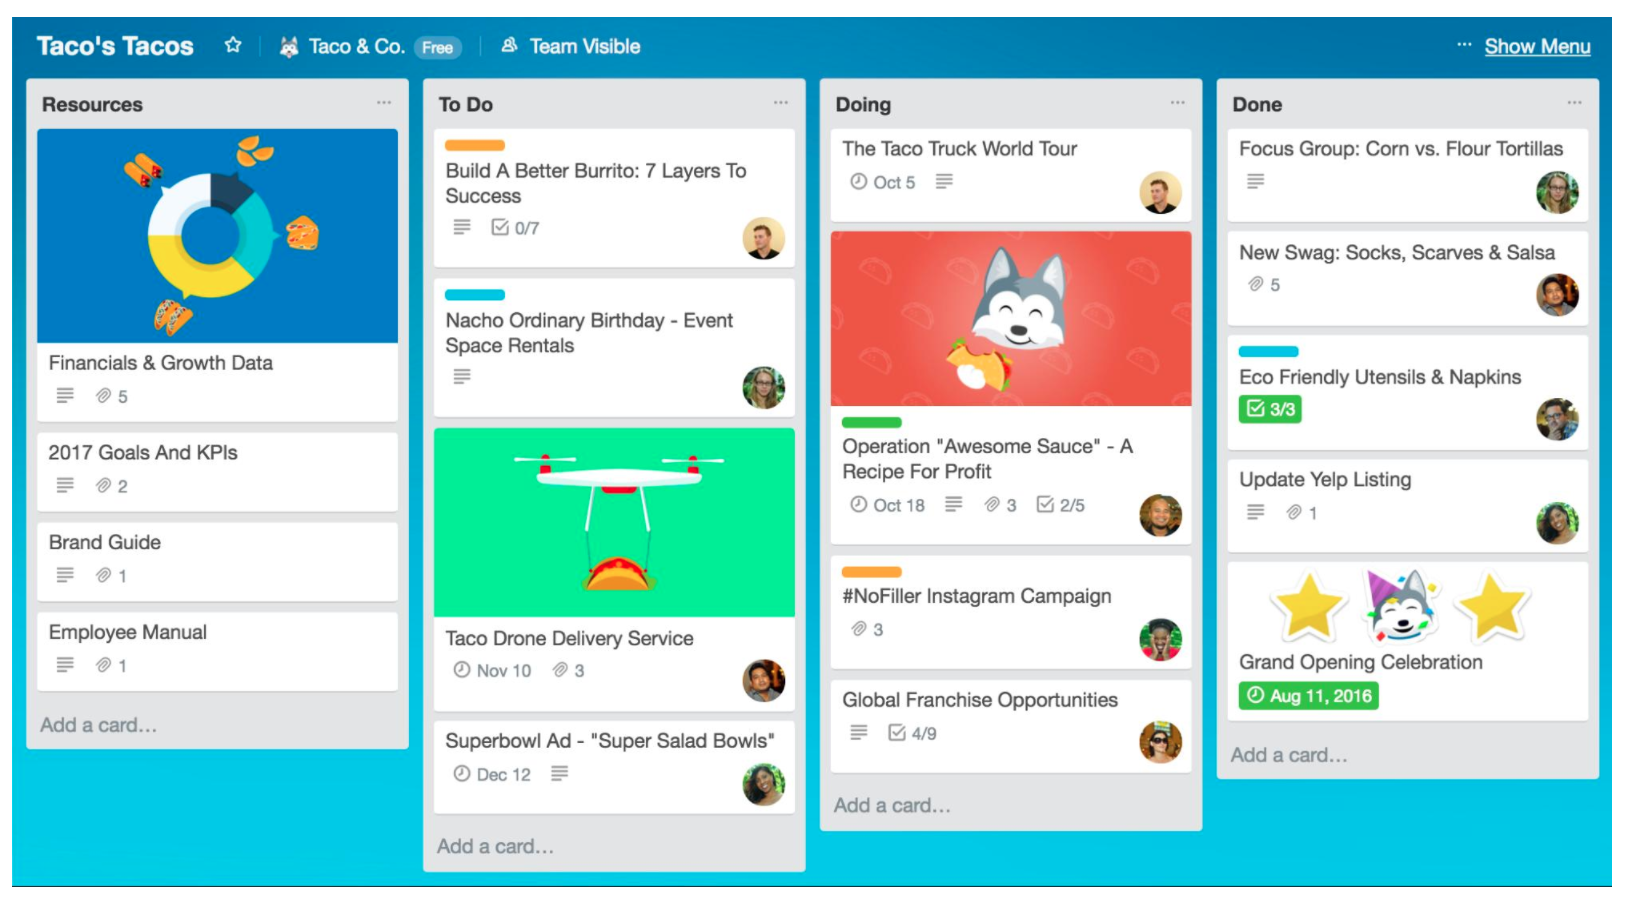
\includegraphics[width=7cm]{figs/trello}}
\caption{Tablero Kanban con Trello}
\end{figure}
\end{frame}



%%---------------------------------------------------------------
\begin{frame}[fragile]
\frametitle{}
\begin{itemize}
\item
Cada tarea, característica o historia de usuario se anota en una
tarjeta o \emph{post-it}, que se va desplazando desde la columna de la izquierda
hasta la columna de la derecha

\item
WIP: \emph{Work in Progress}. Tarjetas que circulan por el tablero.
Es importante minimizar el WIP

\item
El numero de columnas es variable, entre 4 y 7 son valores típicos. La
denominación de cada columna se adapta para cada empresa

Ejemplo:

  \begin{scriptsize}
  \begin{verbatim}
Pendiente | Analizando | En desarrollo | Probando | Aceptado | Producción 
  \end{verbatim}
  \end{scriptsize}
\end{itemize}
\end{frame}


%%---------------------------------------------------------------
\begin{frame}[fragile]
\frametitle{Tarjetas Kanban}

Cada tarjeta tiene

\begin{itemize}
\item
Descripción de la tarea
\end{itemize}


Puede tener:

\begin{itemize}
\item
Quién la está haciendo

\item
Su fecha límite

\item
Distintos colores

\begin{itemize}
\item
Tal vez según la urgencia
\item
Más habitualmente, por el tipo de trabajo

P.e.  Verde: mantenimiento. 
Amarillo: historia de usuario.
Rojo: Bug
\end{itemize}

\item
Indicador de progreso
\end{itemize}

\end{frame}





\section{Problemas}
%%---------------------------------------------------------------
\begin{frame}[fragile]
\frametitle{Diferencias desarrollo-operaciones}
La mayoría de problemas que se  procura resolver con
\emph{DevOps}
parten de que 
normalmente hay diferencias marcadas entre desarrollo
y operaciones. Son equipos muy separados, con
diferente lenguaje, culturas, habilidades, objetivos...

Una de las mayores diferencias es que

\begin{itemize}
\item
Los desarrolladores (analistas, programadores,
\emph{testers} y responsables de calidad)
buscan el cambio continuamente, para corregir errores y añadir
funcionalidad

\item
Los administradores (administradores de sistemas, de bases de datos
y de redes) buscan estabilidad. Ven cualquier cambio como un riesgo
potencial. Nadie les agradecerá la nueva funcionalidad. Pero sí
les culparán de los problemas de explotación provocados
por los cambios

\end{itemize}

\end{frame}



%%---------------------------------------------------------------
\begin{frame}[fragile]
\frametitle{Problemas típicos (1)}
Enumeramos a continuación algunos problemas habituales entre
el equipo de desarrollo y el equipo de operaciones,
que
las técnicas
\emph{DevOps}
buscan solucionar

\begin{itemize}
\item
El software que funcionaba en los equipos de desarrollo, da errores
en producción 

\begin{itemize}
\item
Desarrollo echa la culpa a operaciones

\item
Operaciones echa la culpa a desarrollo
\end{itemize}


\item
Aparece algún problema menor en la funcionalidad o el rendimiento.
El equipo de desarrollo hace un parche rápido sin pasar todos los
controles de calidad
\begin{itemize}
\item
Operaciones instala el parche, arregla una cosa pero rompe otra
\item
Operaciones no instala el parche, porque sabe que los parches son peligrosos 
\end{itemize}

\end{itemize}
\end{frame}


%%---------------------------------------------------------------
\begin{frame}[fragile]
\frametitle{Problemas típicos (2)}
\begin{itemize}
\item
Desarrollo hace un producto de baja calidad, lo mínimo para ser
aceptado


\begin{itemize}
\item
El trabajo ya está \emph{hecho}. El diagrama de Gantt
está cumplido. Los problemas posteriores no importan, son cosa de
 \emph{mantenimiento}, de otro contrato, de otra subcontrata,
de otro presupuesto...

\item
Consumir más recursos (tiempo, esfuerzo) para entregar un producto
de más calidad, no reportará beneficios al equipo de desarrollo
\end{itemize}
\end{itemize}

\end{frame}


%%---------------------------------------------------------------
\begin{frame}[fragile]
\frametitle{Problemas típicos (3)}
\begin{itemize}
\item
Problema contrario al anterior: 
Desarrollo \emph{anancástico} (demasiado perfeccionista)


\begin{itemize}
\item
El equipo de desarrollo prepara un
un software con cambios radicales
(nuevo lenguajes, nuevas librerías).
O preparado para eventualidades poco probables.

\item
Todo lo contrario al \emph{pequeño cambio incremental}.
No tiene en cuenta las implicaciones para operaciones. 
Dispara los costes y/o los plazos, peligrando la viabilidad de la empresa.
A operaciones o al mercado no llegan las soluciones adecuadas
porque la solución \emph{óptima} no está disponible
\end{itemize}
\end{itemize}
\end{frame}


%%---------------------------------------------------------------
\begin{frame}[fragile]
\frametitle{Problemas típicos (4)}
\begin{itemize}
\item
Para intentar evitar los problemas anteriores, se 
\emph{mejora} la especificación de 
los \emph{deliverables} (entregables) que unos proporcionan
a otros


\begin{itemize}
\item
Negociaciones duras,
criterios muy rígidos, contratos
complicados, especificaciones a la defensiva.
Lo fundamental es, en caso de problema, dejar claro 
\emph{quién tiene la culpa}


\item
Esto aumenta los trámites, la preparación y la frecuencia de las entregas

\item
Aumenta la distancia entre los equipos

\end{itemize}
\end{itemize}
\end{frame}


%%---------------------------------------------------------------
\begin{frame}[fragile]
\frametitle{Problemas típicos (5)}
\begin{itemize}
\item
Cultura del héroe
(\emph{rock star, ninja, crack})

\begin{itemize}
\item
Programador individualista. Con frecuencia hace sofware con errores y no documentado.
Aparentemente es muy valioso porque solo él sabe arreglar
esos errores
\end{itemize}

\item
Planificación rígida

\begin{itemize}
\item
Inicialmente se prepara un 
diagrama de Gantt.
Luego todo se fuerza para que encaje en el diagrama
\end{itemize}
\end{itemize}
\end{frame}


\section{Aspectos humanos}
%%---------------------------------------------------------------
\begin{frame}[fragile]
\frametitle{Valores a promover}
\begin{itemize}
\item
Equipos motivados y productivos

\item
Compromiso con objetivos y valores comunes

\item
Respeto al otro

\item
Colaboración bienintencionada entre
las partes/las empresas

\item
Aceptación de un 
cierto ratio
de errores como inevitables, sin buscar culpables
\end{itemize}

Todo esto

\begin{itemize}
\item
Tiene ventajas evidentes
\item
Es difícil de conseguir
\end{itemize}
\end{frame}


%%---------------------------------------------------------------
\begin{frame}[fragile]
\frametitle{Motivación de equipos}
Según Poppendieck, la motivación se puede conseguir con:
% “Lean Software Development” by Mary and Tom Poppendieck

\begin{itemize}
\item
Sensación de pertenencia
\item
Confianza en una cierta tolerancia a los errores
\item
Confianza en la capacidad propia y del resto del equipo
\item
Celebración conjunta de los progresos

\begin{itemize}
\item
Teniendo en cuenta que no todo el mundo sale de copas o juega
al Paintball
\end{itemize}
\end{itemize}
\end{frame}


%%---------------------------------------------------------------
\begin{frame}[fragile]
\frametitle{Trabajo en equipo productivo}
\begin{itemize}
\item
Definir objetivos, métodos, pasos, plazos temporales... y reajustarlo cuando sea necesario

\item
Evitar la microgestión.
Que los gestores digan qué hacer, pero sin demasiados detalles del cómo. 
El equipo se auto-organiza

\begin{itemize}
\item
Esto suele ser más eficiente
\item
Hace al equipo sentirse más valorado
\end{itemize}
\end{itemize}
\end{frame}

%%----------------------------------------------
\begin{frame}[fragile]
\begin{itemize}
\item
Hacer pequeños experimentos. Fallar a menudo pero pronto y con pequeñas cosas

\item
De vez en cuando (una vez al día, a la semana...) reservar un rato para alguien de operaciones
se siente con alguien de desarrollo

\item
Evitar el \emph{presentismo laboral}. 
Respetar el equilibrio entre el trabajo y la vida personal.
No esperar que los empleados hagan jornadas maratonianas
en la oficina y que luego contesten al correo a cualquier hora

\end{itemize}
\end{frame}

%%---------------------------------------------------------------
\begin{frame}[fragile]
\frametitle{Comunicación efectiva}
Que los individuos y equipos:
\begin{itemize}
\item

Comprendan las circustancias y dificultades de los demás

\item
Busquen influenciar en otros de forma positiva.

No porque \emph{te lo mando} o \emph{me debes una}, sino porque
esto es lo mejor para todos

\item
Reconozcan  el trabajo ajeno. Hacerlo en público es mucho más
efectivo. Y si hay que hacer algún reproche, con mucha
mano izquierda y en privado

\end{itemize}
\end{frame}

%%----------------------------------------------
\begin{frame}[fragile]

Reuniones de calidad

\begin{itemize}
\item
Todos los convocados llegan puntuales. La reunión acaba puntualmente

\item
Meta-decisiones claras. Ya sea por
jerarquía, por votación, o idealmente, por consenso

\item
Los participantes hablan de uno en uno

\item
Lo que solo afecta a unos pocos, no se trata en el tiempo de todos

\item
...

\end{itemize}

Sin olvidar las

\begin{itemize}
\item
Discusiones retrospectivas.
Reuniones con periodicidad predeterminada para tratar
las etapas superadas, para analizarlas
y extraer conclusiones.

\item
Reuniones \emph{post morten}. Similares a las retrospectivas,
pero provocadas por un problema concreto.
Siempre es necesario trabajar de forma constructiva  sin echar la culpa a nadie,
pero en estos casos, mas que nunca.
\end{itemize}
\end{frame}

\section{Aspectos técnicos}


%%---------------------------------------------------------------
\begin{frame}[fragile]
\frametitle{Automatización}
La automatización es una técnica fundamental en 
\emph{DevOps}

Tareas que se pueden automatizar:

\begin{itemize}
\item
Construcción (compilación)
\item
Pruebas
\item
Despliegue (puesta en producción)
\item
Configuración en los distintos entornos
\item
Monitorización
\item
Control de incidencias
\end{itemize}

Ultimamente se ha introducido el término \emph{orquestar}:

\begin{itemize}
\item
Automatizar 

Usar herramientas (scripts o similares) que permitan realizar una tarea sin intervención de una persona

\item
Orquestar 

Coordinar diversas automatizaciones de tareas individuales, para que formen procesos / flujos de trabajo
\end{itemize}
\end{frame}

%%---------------------------------------------------------------
\begin{frame}[fragile]
\frametitle{}
Automatizar (incluyendo orquestar) es, en general, positivo. Con algunas salvedades

\begin{itemize}
\item
Debemos asegurarnos de que merezca la pena. Que el esfuerzo
necesario para preparar y mantener la automatización, sea menor
que el esfuerzo de realizar las tareas a mano.

\item
Paradoja del exceso de automatización

Inevitablemente, habrá ocasiones en que el sistema requiera intervención
humana (errores, cambios no previstos...).
Cuánto más automatizado esté el sistema:

\begin{itemize}
\item
Más complejos serán estos cambios, más especializado
tendrá que ser el personal

\item
Menos especializado será el personal del día a día.

\emph{Como esto lo puede llevar cualquiera, el resultado es que lo acaba
llevando cualquiera}
\end{itemize}
\end{itemize}
\end{frame}


%%---------------------------------------------------------------
\begin{frame}[fragile]
\frametitle{Técnicas de despliegue (1)}
\begin{itemize}
\item
Despliegue frecuente

Un cambio grande puede ser muy drástico. Por el contrario, el 
despliegue frecuente pone
en producción pequeños cambios, de forma continua

\begin{itemize}
\item
Esto familiariza a todo el equipo con el proceso de introducir novedades

\item
Los cambios menores implican problemas potenciales menores

\item
Hay técnicas más avanzadas (integración continua, entrega continua, despliegue continuo).
Pero realizar al menos 
\emph{despliegue frecuente}
es prácticamente imprescindible dentro de la filosofía
\emph{DevOps}
\end{itemize}

\end{itemize}
\end{frame}
%%----------------------------------------------
\begin{frame}[fragile]
\frametitle{Técnicas de despliegue (2)}
\begin{itemize}
\item
Conmutación de funciones

Ejemplo:
Ponemos en producción funcionalidad nueva. Pero si falla
y decidimos desactivarla, se puede hacer con un conmutador
sencillo desde el código. Sin necesidad de volver a desplegar
el código \emph{viejo}


\begin{itemize}
\item
Los contenedores pueden hacer innecesaria esta técnica
\end{itemize}

\item
\emph{Dark Launching}

Las nuevas versiones se aplican solo a unos pocos usuarios

\begin{itemize}
\item
Esto facilita la corrección de problemas y limita los problemas potenciales
\item
Pueden ser los empleados, pueden ser voluntarios, pueden ser usuarios
que hemos detectado como \emph{avanzados} o pueden ser aleatorios
\end{itemize}


\end{itemize}
\end{frame}
%%----------------------------------------------
\begin{frame}[fragile]
\frametitle{Técnicas de despliegue (3)}
\begin{itemize}
\item
\emph{Blue Green Deployment}

La versión nueva y la versión anterior se preparan para que funcionen
en paralelo 

\begin{itemize}
\item
Para conmutar de la
\emph{versión azul}
a la
\emph{versión verde}
no hay que cambiar el código, solo el router/el
\emph{balanceador} de carga o algún fichero de configuración
\end{itemize}
\end{itemize}
\end{frame}

%%---------------------------------------------------------------
\begin{frame}[fragile]
\frametitle{Integración, entrega y despliegue continuo}

Las siguiente técnicas son habituales en 
\emph{DevOps},
aunque

\begin{itemize}
\item
No son imprescindibles para hacer 
\emph{DevOps}
\item
Implementarlas no significa estar haciendo
\emph{DevOps}
\end{itemize}

En cualquier entorno de desarrollo moderno de cierto tamaño, hay varios desarrolladores,
utilizando un sistema de control de versiones. Cada uno tiene su copia de trabajo del software,
que con cierta periodicidad, integra en el repositorio principal

\begin{itemize}
\item
\emph{Continuous Integration} (CI) 

Realizar esta integración muy a menudo. Típicamente
varias veces al día

\end{itemize}
\end{frame}
%%----------------------------------------------
\begin{frame}[fragile]
\begin{itemize}
\item
\emph{Continuous Delivery} (CD) 

No solamente hacer
\emph{Continuous Integration}, sino dar un paso más allá. Además de integrar el código, asegurarse
de que está listo para ponerse en producción muy a menudo. Esto es, pasar los controles de calidad
y automatizar la puesta en producción. Tal vez no tan a menudo como la CI, pero sí
muy a menudo. P.e. una vez al día.

\item
\emph{Continuous Deployment} 

No solo hacer 
\emph{Continuous Delivery}, sino dar un paso más allá. Además de asegurarse de que el código tiene
calidad como para ponerse en producción, ponerlo realmente en producción
\end{itemize}
\end{frame}


\section{Herramientas}
%%---------------------------------------------------------------
\begin{frame}[fragile]
\frametitle{Herramientas}
Las siguientes herramientas son habituales cuando se siguen los
principios
\emph{DevOps}
\begin{itemize}
\item
Contenedores Docker

\begin{tiny}
\url{https://gsyc.urjc.es/~mortuno/lagrs/02-virtualizacion_I.pdf}
\end{tiny}

\begin{tiny}
\url{https://gsyc.urjc.es/~mortuno/lagrs/02-virtualizacion_III.pdf}
\end{tiny}

\item
Ansible

\item
Jenkins

\item
Vagrant

\end{itemize}

\end{frame}


%%---------------------------------------------------------------
\begin{frame}[fragile]
\frametitle{Jenkins}
\begin{figure}
\centerline{
\includegraphics[width=5cm]{figs/logo_jenkins}}
%\caption{}
\url{https://jenkins.io}
\end{figure}

Jenkins es una herramienta para implementar
Integración Continua (C.I.)
\begin{itemize}
\item
Aparece en el año 2011. Es software libre, muy popular

\item
Aplicación basada en web

\end{itemize}
\end{frame}
%%----------------------------------------------
\begin{frame}[fragile]
\begin{itemize}
\item
Va un paso más allá de herramientas como Maven, que construyen
el fuente pero no hacen C.I.

\item
Su entorno nativo es Java, pero tiene
\emph{plugins} para distintos lenguajes,
herramientas de control de versiones, de virtualización, de testing, de
comunicación con el personal, etc

\item
La unidad principal es el 
\emph{build}: el conjunto de pasos para desplegar una aplicación software 

\begin{itemize}
\item
Un \emph{build}
se pueden disparar manualmente, por un commit, o
con planificación periódica similar a cron

\item
Un \emph{build}
se organiza  en
\emph{pipelines},
cada una compuesta de
\emph{steps}
\end{itemize}
\end{itemize}

\end{frame}
%%----------------------------------------------
\begin{frame}[fragile]

  \begin{scriptsize}
  \begin{verbatim}
Jenkinsfile (Declarative Pipeline)
pipeline {
    agent any
    stages {
        stage('Build') {
            steps {
                echo 'Building'
            }
        }
        stage('Test') {
            steps {
                echo 'Testing'
            }
        }
        stage('Deploy') {
            steps {
                echo 'Deploying'
            }
        }
    }
}
  \end{verbatim}
  \end{scriptsize}
\end{frame}


%%---------------------------------------------------------------
\begin{frame}[fragile]
\frametitle{Vagrant}


\begin{figure}
\centerline{
\includegraphics[width=6cm]{figs/logo_vagrant}}
%\caption{}
\url{https://www.vagrantup.com}
\end{figure}


\begin{itemize}
\item
Es una herramienta para construir y gestionar entornos de
máquinas virtuales.

\item
Creado en 2010, es software libre, muy popular

\item
Funciona sobre
Linux, FreeBSD, macOS, y Microsoft Windows
\end{itemize}
\end{frame}

%%----------------------------------------------
\begin{frame}[fragile]
\begin{itemize}
\item
Soporta las principales plataformas de virtualización:
Docker, VirtualBox, VMware, AWS, Azure,  entre otras

\item
Su función básica es reemplazar el interfaz gráfico de estas
plataformas, proporcionando un interfaz de texto,
programable y homogéneo que permite preparar las máquinas, levantarlas,
configurarlas, etc

\item
Para la configuración, se integra con Ansible, Chef y Puppet, entre otras
\end{itemize}
\end{frame}



%%---------------------------------------------------------------
\begin{frame}[fragile]
\frametitle{Ansible}
\begin{figure}
\centerline{
\includegraphics[width=3cm]{figs/logo_ansible}}
%\caption{}
\url{https://www.ansible.com}
\end{figure}

Ansible es un software de gestión de configuraciones


\begin{itemize}
\item
Creado por
Michael DeHaan en 2012. En la actualidad pertenece a RedHat 

\item
Sofware libre, muy popular

\item
Arquitectura cliente servidor

\end{itemize}
\end{frame}
%%----------------------------------------------
\begin{frame}[fragile]

\begin{itemize}
\item
 Los clientes se denominan
\emph{nodos}. Son las máquinas controladas. 
Solo necesitan un servidor de ssh, por tanto
soporta cualquier Linux, Unix, MacOS. También funciona sobre la 
PowerShell de Microsoft Windows

\item
El servidor se denomina
\emph{controlling machine}. Es la máquina que administra y controla los nodos.
El soporte nativo es para 
Linux.  Hay versiones para MacOS y otras plataformas, prácticamente
cualquiera donde funcione python y pip

\item
Ansible sigue un 
paradigma \emph{push}: el controlador envía las órdenes
vía ssh

\begin{itemize}
\item
Otras herramientas similares 
como \emph{puppet} tienen
un enfoque
\emph{pull}, 
que resulta más complejo:
la máquina administrada corre un demonio que, periódicamente, se
\emph{trae} las órdenes
\end{itemize}

\end{itemize}
\end{frame}
%%----------------------------------------------
\begin{frame}[fragile]
\frametitle{Conceptos principales en Ansible}

\begin{itemize}
\item
\emph{Inventory}

Fichero que contiene el listado de las máquinas administradas,
con su nombre y/o dirección IP, puerto, claves ssh, etc

\item
\emph{Playbook}

Es una especie de \emph{howto} automatizable, un script de propósito
específica (configurar una máquina), de  alto 
nivel y fácilmente legible por humanos

\begin{itemize}
\item
Palabra inglesa que significa 
libro de juego, libro de tácticas o libro de reglas

\item
Escrito en formato YAML, similar a JSON pero con sintaxis pensada
para que sea cómodo para las personas. Filosofía análoga
al formato 
\emph{markdown}, pero para datos, no para texto
\end{itemize}

\item
\emph{Role}

Estructura de nivel superior al
\emph{playbook}.
Permite hacer plantillas de \emph{playbooks}.
Está formado por
\emph{playbooks}, ficheros,
dependencias entre
\emph{playbooks}...


\end{itemize}
\end{frame}
%%----------------------------------------------
\begin{frame}[fragile]

\emph{Ansible Galaxy}

Repositorio centralizado de roles.
Facilita la instalación de software. Equivalente a tener
un repositorio de libros de instrucciones, pero que se autoejecutan


\url{https://galaxy.ansible.com}
\end{frame}

%%---------------------------------------------------------------
\begin{frame}[fragile]
\frametitle{}

  \begin{scriptsize}
  \begin{verbatim}
# Configurar un servidor web básico con  nginx
- name: Configurar servidor web con nginx
  hosts: miServidor01
  sudo: yes
  tasks:
    - name: install nginx
      apt: name=nginx update_cache=yes

    - name: copy nginx conf file
      copy: src=files/nginx.conf dest=/etc/nginx/nginx.conf

    - name: copy nginx server file
      copy: src=files/server.conf dest=/etc/nginx/sites-available/default

    - name: enable config
      file: >
        dest=/etc/nginx/conf.d/default
        src=/etc/nginx/sites-available/default
        state=link
    - name: copy index.html
      template: src=templates/index.html.j2 dest=/usr/share/nginx/html/index.html mode=0644

    - name: restart nginx
      service: name=nginx state=restarted enabled=yes
  \end{verbatim}
  \end{scriptsize}
\end{frame}


%%---------------------------------------------------------------
\begin{frame}[fragile]
\frametitle{}
\begin{itemize}
\item
El guión denota un elemento de una lista (una tarea, (\emph{task})

\item
Cada tarea suele estar compuesta por varias líneas.

La primera suele ser el nombretiene un nombre (opcional)

A continuación, la orden


p.e.

\verb|apt: name=nginx update_cache=yes|

ejecutará en cada nodo

\verb|apt update; apt install -y nginx|

%La barra | respeta las nuevas líneas
%el símbolo de mayor hace que se ignoren los saltos de línea

\end{itemize}

\end{frame}


%%---------------------------------------------------------------
\begin{frame}[fragile]
\frametitle{Referencias}
\begin{itemize}
\item[[1]]
\emph{DevOps for Developers}

Michael Huttermann. Ed. Apress, 2012

\begin{tiny}
\url{http://proquest.safaribooksonline.com/book/software-engineering-and-development/9781430245698}
\end{tiny}

\item[[2]]
\emph{Effective DevOps: Building a Culture of Collaboration, Affinity, and Tooling at Scale}

Jennifer Davis, Katherine Daniels. Ed. O'Reilly, 2016

\begin{tiny}
\url{http://proquest.safaribooksonline.com/book/software-engineering-and-development/9781491926291}
\end{tiny}

\item[[3]]
\emph{DevOps for Web Development}

Mitesh Soni.
Ed. Pack, 2016.

\begin{tiny}
\url{http://proquest.safaribooksonline.com/book/web-design-and-development/9781786465702}
\end{tiny}


\item[[4]]
\emph{DevOps: A Software Architect's Perspective}

Len Bass, Ingo Weber, Liming Zhu.
Ed. Pearson, 2015

\begin{tiny}
\url{http://proquest.safaribooksonline.com/book/software-engineering-and-development/9780134049885}
\end{tiny}
\end{itemize}
\end{frame}


%%---------------------------------------------------------------
\begin{frame}[fragile]
\frametitle{}
\begin{itemize}
\item[[5]]
\emph{Kanban in Action}

Marcus Hammarberg, Joakim Sunden. Ed. Manning, 2014

\begin{tiny}
\url{http://proquest.safaribooksonline.com/book/software-engineering-and-development/agile-development/9781617291050}
\end{tiny}

\item[[6]]
\emph{The Elements of Scrum}

Chris Sims, Hillary Louise Johnson. Ed. Dymaxicon, 2011
\end{itemize}

\end{frame}


\end{document}
